\documentclass[a4paper, 11pt]{article}           %{{{1
% basic packages                                  {{{2
\usepackage[T1]{fontenc}
\usepackage[scaled=0.975]{helvet}
\usepackage[utf8]{inputenc}
\usepackage{amsmath}
\usepackage{lastpage}
\usepackage{graphicx}
\usepackage{amsfonts}
\usepackage{variations}
\usepackage{pgf,tikz}           % dessin
\usepackage{mathrsfs}
\usetikzlibrary{arrows}
\usepackage{pgfkeys}        % fenetrage des plot TikZ
\usepackage{yhmath}         % arc au dessus des lettres
\usepackage{calc}           % calcul de longueur
\usepackage{variations}     % tableau de variations
\usepackage{multicol}
\usepackage{enumitem}
% ==== PROGRAMMATION
\usepackage{xcolor}                                                             %
\usepackage{listings}                                                           %
% listings                                        {{{3
\definecolor{mygreen}{rgb}{0,0.6,0}
\definecolor{mygray}{rgb}{0.5,0.5,0.5}
\definecolor{mymauve}{rgb}{0.58,0,0.82}
\definecolor{deepblue}{rgb}{0,0,0.5}
\definecolor{deepred}{rgb}{0.6,0,0}
\definecolor{deepgreen}{rgb}{0,0.5,0}
\lstset{%
%       backgroundcolor=\color{white},   % choose the background color; you must add \usepackage{color} or \usepackage{xcolor}; should come as last argument
        basicstyle=\footnotesize,        % the size of the fonts that are used for the code
%       breakatwhitespace=false,         % sets if automatic breaks should only happen at whitespace
%       breaklines=true,                 % sets automatic line breaking
%       captionpos=b,                    % sets the caption-position to bottom
        commentstyle=\color{mygreen},    % comment style
%       deletekeywords={type},           % if you want to delete keywords from the given language
%       emph={},                         % Custom highlighting
%       emphstyle=\ttb\color{deepred}    % Custom highlighting style
%       escapeinside={\%*}{*)},          % if you want to add LaTeX within your code
%       extendedchars=true,              % lets you use non-ASCII characters; for 8-bits encodings only, does not work with UTF-8
        frame=shadowbox,                 % adds a frame around the code {single, shadowbox}
%       keepspaces=true,                 % keeps spaces in text, useful for keeping indentation of code (possibly needs columns=flexible)
        keywordstyle=\color{blue},       % keyword style
	language=Python,                 % the language of the code {Python, C}
%       morekeywords={*,...},            % if you want to add more keywords to the set
        numbers=left,                    % numbers = (none, left, right)
%       numbersep=5pt,                   % how far the line-numbers are from the code
%       numberstyle=\tiny\color{mygray}, % the style that is used for the line-numbers
%       otherkeywords={self},            % Add keywords here
%       rulecolor=\color{black},         % if not set, the frame-color may be changed on line-breaks within not-black text (e.g. comments (green here))
	rulesepcolor=\color{gray}        % shadowbox color
%       showspaces=false,                % show spaces everywhere adding particular underscores; it overrides 'showstringspaces'
%       showstringspaces=false,          % underline spaces within strings only
%       showtabs=false,                  % show tabs within strings adding particular underscores
%       stepnumber=1,                    % the step between two line-numbers. If it's 1, each line will be numbered
%       stringstyle=\color{mymauve},     % string literal style
%       tabsize=4,                       % sets default tabsize to 2 spaces
%       title=\lstname                   % show the filename of files included with \lstinputlisting; also try caption instead of title
}
%}}}
%}}}

% mise en page                                    {{{2
\addtolength{\voffset}{-1.8cm}
\addtolength{\textheight}{4cm}
\addtolength{\hoffset}{-2.5cm}
\addtolength{\textwidth}{4cm}
\addtolength{\headsep}{-0.5cm}
\usepackage{fancyhdr}
\setlength{\headheight}{14.00pt}
\pagestyle{fancy} % Numérotation des pages
\renewcommand\headrulewidth{1pt}
\fancyhead[L]{BP SN}
\fancyhead[C]{micro:bit}
\fancyhead[R]{introduction - suite}
\renewcommand\footrulewidth{1pt}
\fancyfoot[L]{v 1.2 -- J.B.}
\fancyfoot[C]{\textbf{domotique, syst. embarqués \& de gestion de l'habitat}}
\fancyfoot[R]{\thepage/\pageref{LastPage}}
%\lhead{3E}%haut de page gauche
%}}}

% Compteurs:                                     {{{2
\addtocounter{page}{0}
\newcounter{Q}
\newcounter{exoNB}
%}}}

% Longueur:                                      {{{2
\newlength{\longueurA}
\newlength{\longueurB}
\setlength{\parindent}{0pt}
\setlength{\parskip}{2pt}
\renewcommand{\baselinestretch}{1}
%}}}

% newcommand                                     {{{2
\newcommand{\objectif}[1]{\textsc{\huge #1} }
\newcommand{\partie}[1]{\textsc{\huge #1} }
\newcommand{\question}{\stepcounter{Q} $\boxed{\arabic{Q}}$ }
\newcommand{\ligne}{\underline{\hspace{ \textwidth}} }
\newcommand{\LIGNE}{\vspace{2mm}\underline{\hspace{ \textwidth}} }
\newcommand{\reponse}{
  \par\nobreak
  \noindent\rule{0pt}{1.5\baselineskip}% Provides a larger gap between the preceding paragraph and the dots
  {\noindent\makebox[\linewidth]{\dotfill}\endgraf}% ... dotted lines ...
% \bigskip% Gap between dots and next paragraph
  }
\newcommand{\exo}[1]{\stepcounter{exoNB}\textsc{\Large Exercice \arabic{exoNB} -- #1} }
\newcommand{\EXO}[2]{\stepcounter{exoNB}\textsc{\Large Exercice \arabic{exoNB} -- #1} \hfill \textbf{#2 points}}
\newcommand{\pb}[1] {\stepcounter{exoNB}\textsc{\Large Problème \arabic{exoNB} -- #1} }
\newcommand{\PB}[2] {\stepcounter{exoNB}\textsc{\Large Problème \arabic{exoNB} -- #1} \hfill \textbf{#2 points}}
%}}}

% Divers                                          {{{2
% listings                                        {{{3
%\definecolor{mygreen}{rgb}{0,0.6,0}
%\definecolor{mygray}{rgb}{0.5,0.5,0.5}
%\definecolor{mymauve}{rgb}{0.58,0,0.82}
%\definecolor{deepblue}{rgb}{0,0,0.5}
%\definecolor{deepred}{rgb}{0.6,0,0}
%\definecolor{deepgreen}{rgb}{0,0.5,0}
%\lstset{%
%        backgroundcolor=\color{white},   % choose the background color; you must add \usepackage{color} or \usepackage{xcolor}; should come as last argument
%        basicstyle=\footnotesize,        % the size of the fonts that are used for the code
%        breakatwhitespace=false,         % sets if automatic breaks should only happen at whitespace
%        breaklines=true,                 % sets automatic line breaking
%        captionpos=b,                    % sets the caption-position to bottom
%        commentstyle=\color{mygreen},    % comment style
%        deletekeywords={...},            % if you want to delete keywords from the given language
%        escapeinside={\%*}{*)},          % if you want to add LaTeX within your code
%        extendedchars=true,              % lets you use non-ASCII characters; for 8-bits encodings only, does not work with UTF-8
%        frame=single,                    % adds a frame around the code
%        keepspaces=true,                 % keeps spaces in text, useful for keeping indentation of code (possibly needs columns=flexible)
%        keywordstyle=\color{blue},       % keyword style
%        morekeywords={*,...},            % if you want to add more keywords to the set
%        numbers=left,                    % where to put the line-numbers; possible values are (none, left, right)
%        numbersep=5pt,                   % how far the line-numbers are from the code
%        numberstyle=\tiny\color{mygray}, % the style that is used for the line-numbers
%        rulecolor=\color{black},         % if not set, the frame-color may be changed on line-breaks within not-black text (e.g. comments (green here))
%        showspaces=false,                % show spaces everywhere adding particular underscores; it overrides 'showstringspaces'
%        showstringspaces=false,          % underline spaces within strings only
%        showtabs=false,                  % show tabs within strings adding particular underscores
%        stepnumber=2,                    % the step between two line-numbers. If it's 1, each line will be numbered
%        stringstyle=\color{mymauve},     % string literal style
%        tabsize=4,                       % sets default tabsize to 2 spaces
%        title=\lstname                   % show the filename of files included with \lstinputlisting; also try caption instead of title
%}
%\lstset{%
%        language=Python,                 % the language of the code
%        otherkeywords={self},            % Add keywords here
%        deletekeywords={type},           % if you want to delete keywords from the given language
%        emph={},                         % Custom highlighting
%        emphstyle=\ttb\color{deepred}    % Custom highlighting style
%}
%}}}

% PRL style line                                 {{{3
\newlength{\diamondrulelength}
\setlength{\diamondrulelength}{0.6\textwidth}
\newlength{\diamondrulethickness}
\setlength{\diamondrulethickness}{2pt}
\newcommand{\diamondrule}{\begin{center}\tikz{\fill[black] (0.5\diamondrulelength,0) -- (0,0.5\diamondrulethickness) -- (-0.5\diamondrulelength,0) -- (0,-0.5\diamondrulethickness) -- cycle;}\end{center}}
%}}}

% fixed with tabular                             {{{3
\usepackage{array}
\newcolumntype{L}[1]{>{\raggedright\let\newline\\\arraybackslash\hspace{0pt}}m{#1}}
\newcolumntype{C}[1]{>{\centering\let\newline\\\arraybackslash\hspace{0pt}}m{#1}}
\newcolumntype{R}[1]{>{\raggedleft\let\newline\\\arraybackslash\hspace{0pt}}m{#1}}
%}}}

%}}}
%}}}

\begin{document}
\sffamily
\objectif{Objectif :\\programmation d'un micro-controleur}\\


\partie{Le matériel} \\ %{{{1
- 10 cases contenant 10 {micro:bits \& 20 docs (safety guide \& guide de démarrage)}\\
- 5 cases contenant 10 boitiers pour pile \\
- 5 cases contenant 10 adaptateurs USB\\
- 4 cases contenant 20 piles AAA
\begin{center}
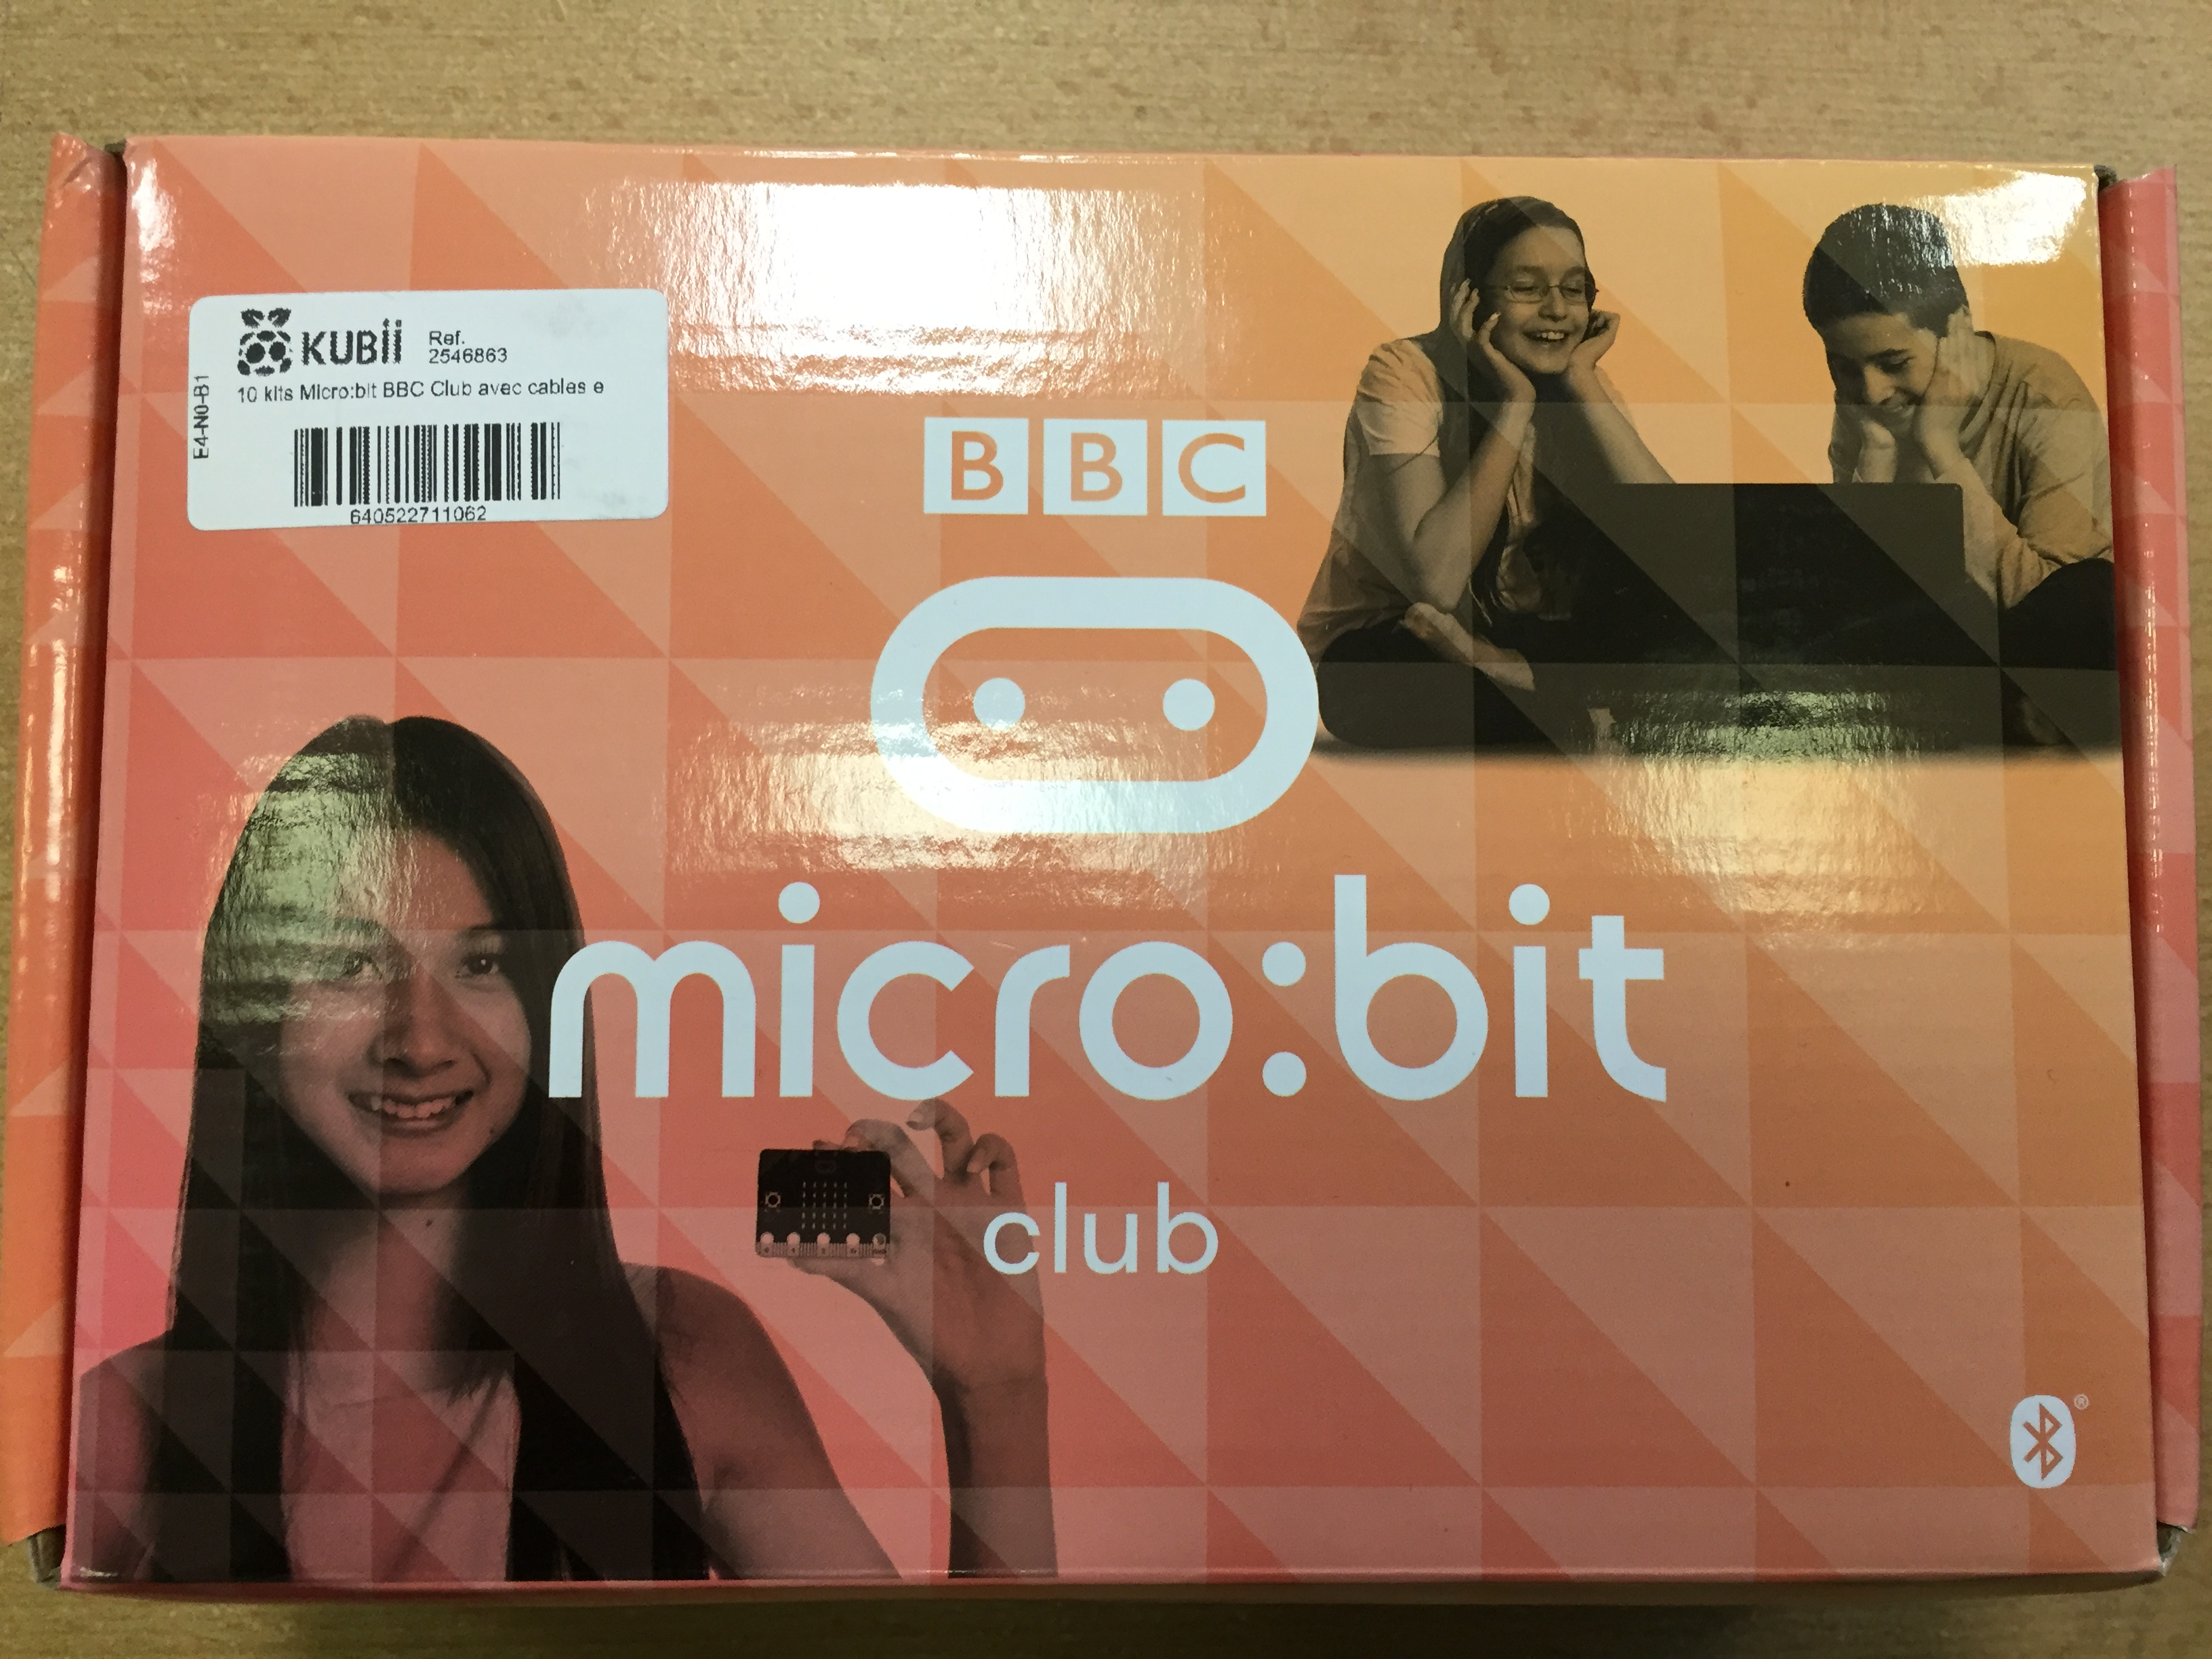
\includegraphics[width=0.45\textwidth]{boite_fermee}
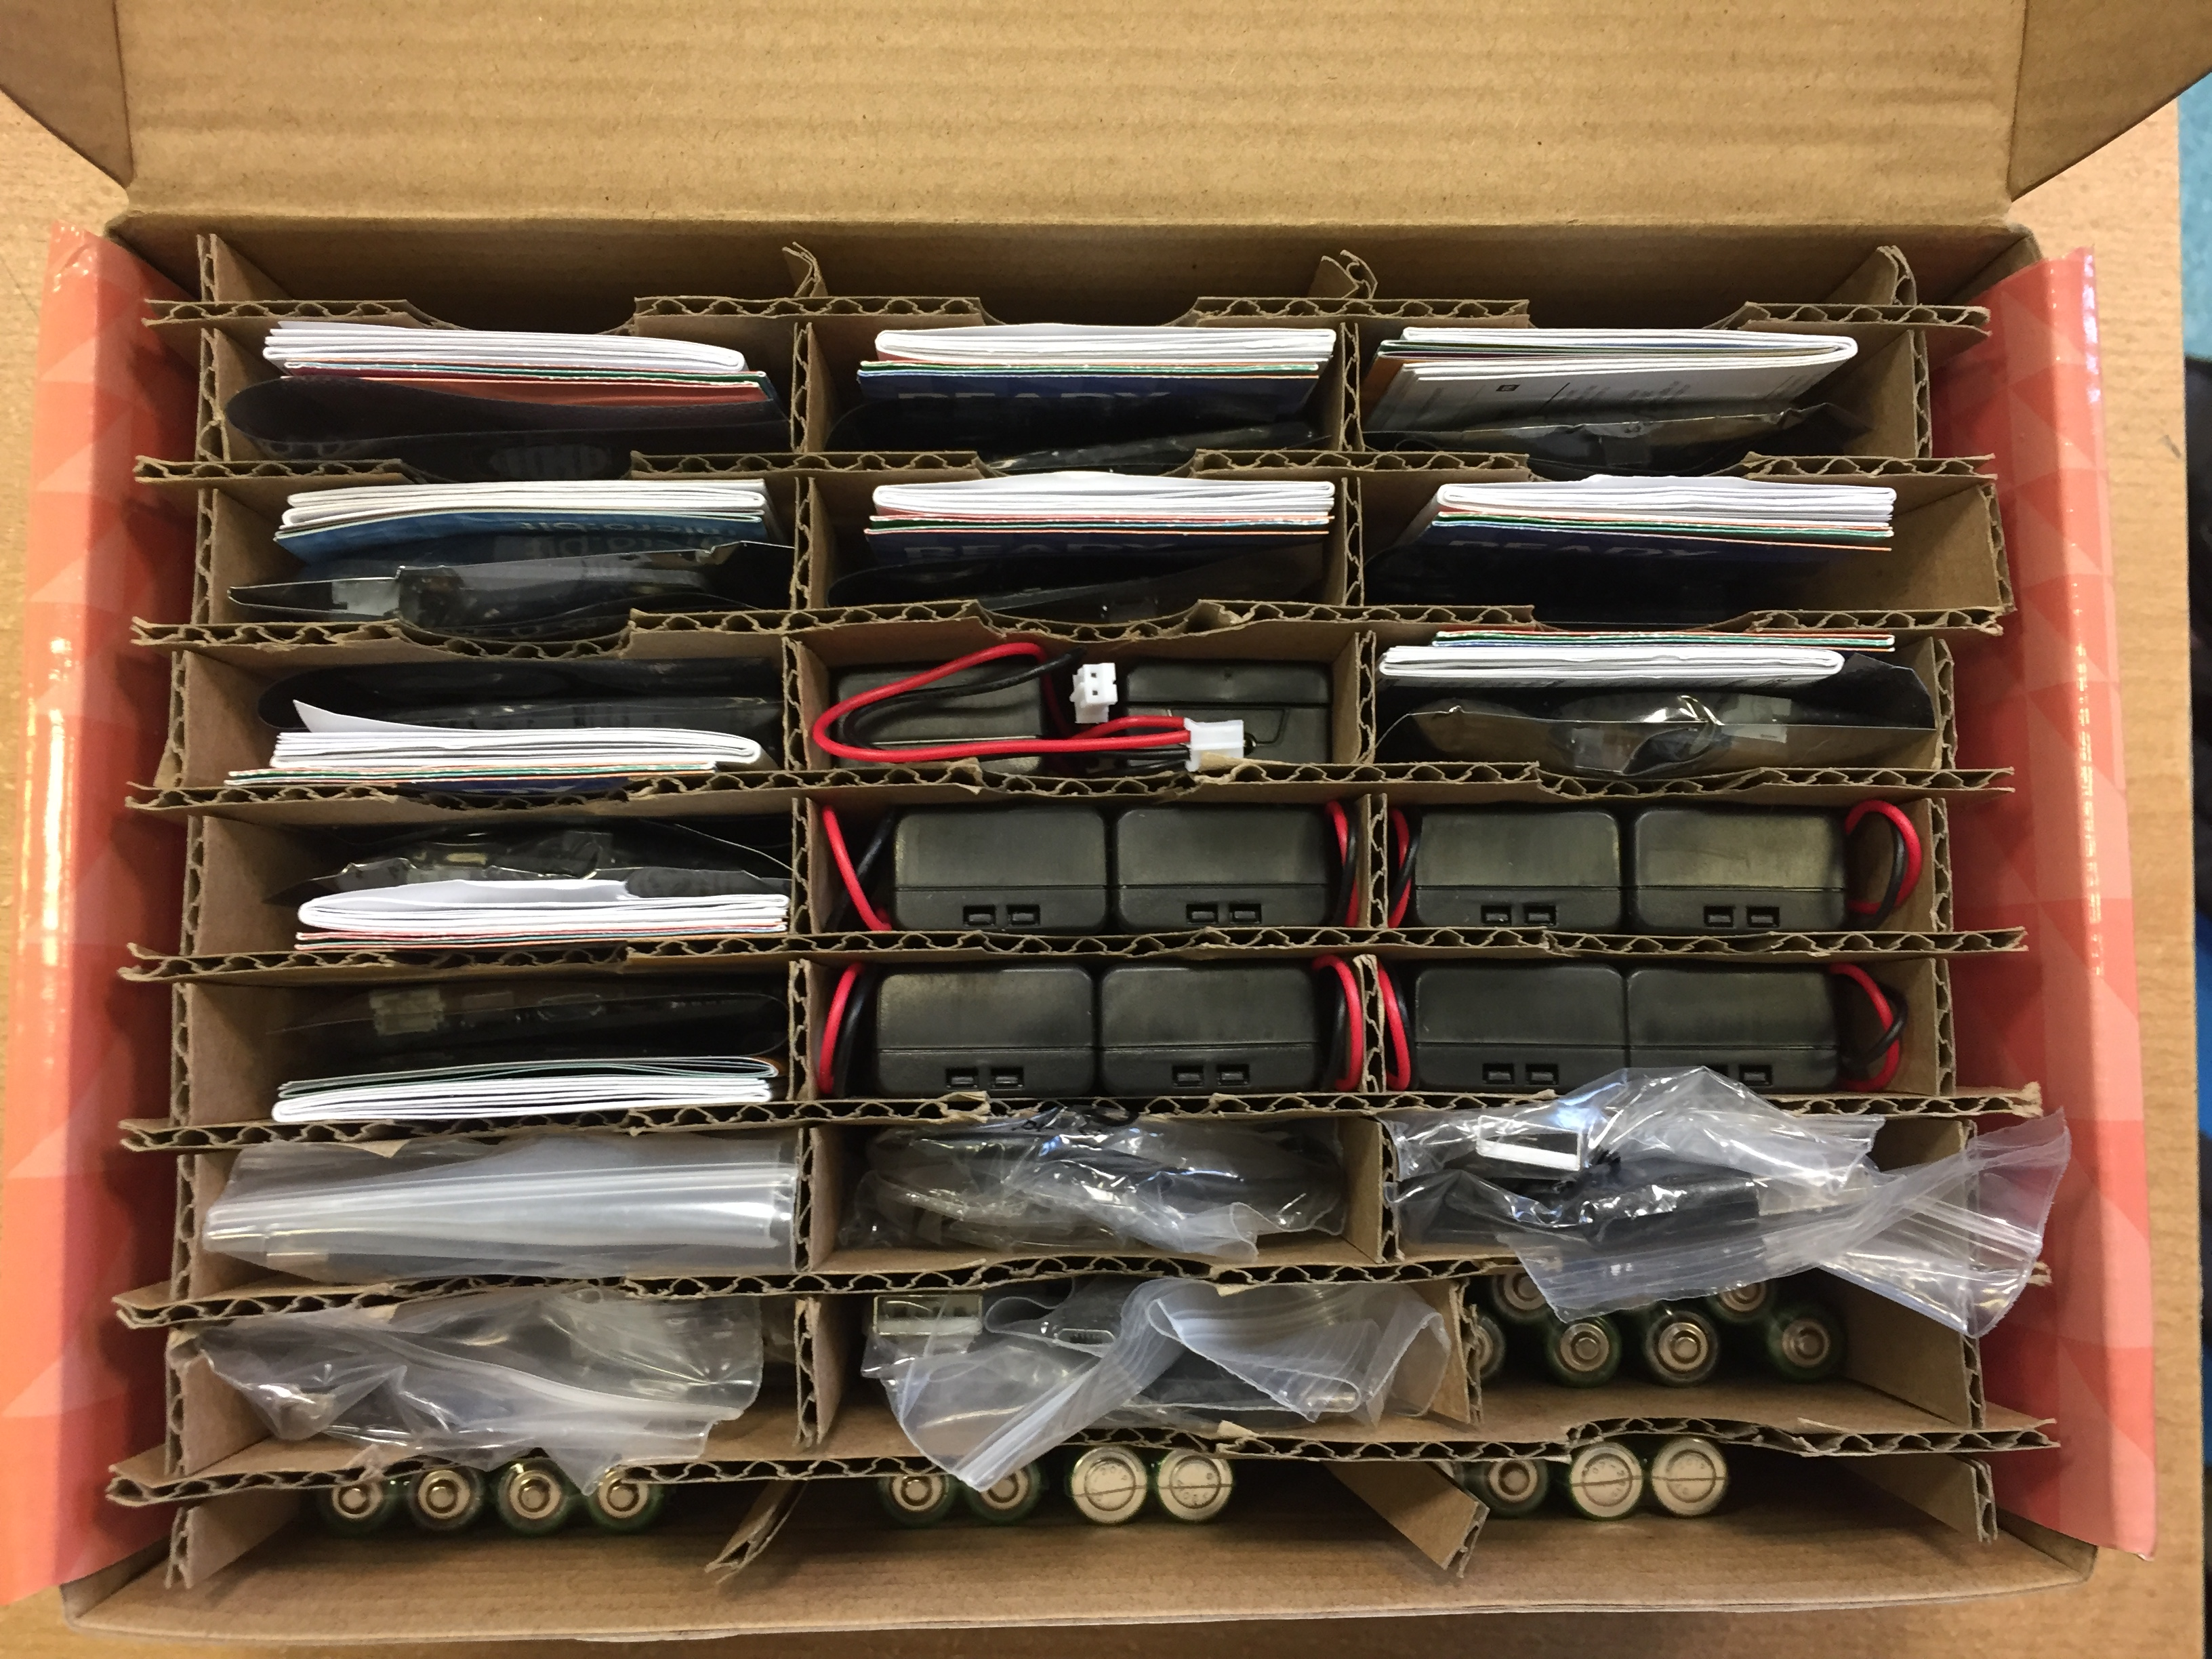
\includegraphics[width=0.45\textwidth]{boite_ouverte}
\end{center}
%}}}

\partie{Rappels : environnement de développement} \\
Ouvrir \texttt{http://python.microbit.org/v/1} pour accéder l'environnement suivant utilisé dans le TP précédent.\\
\begin{center}
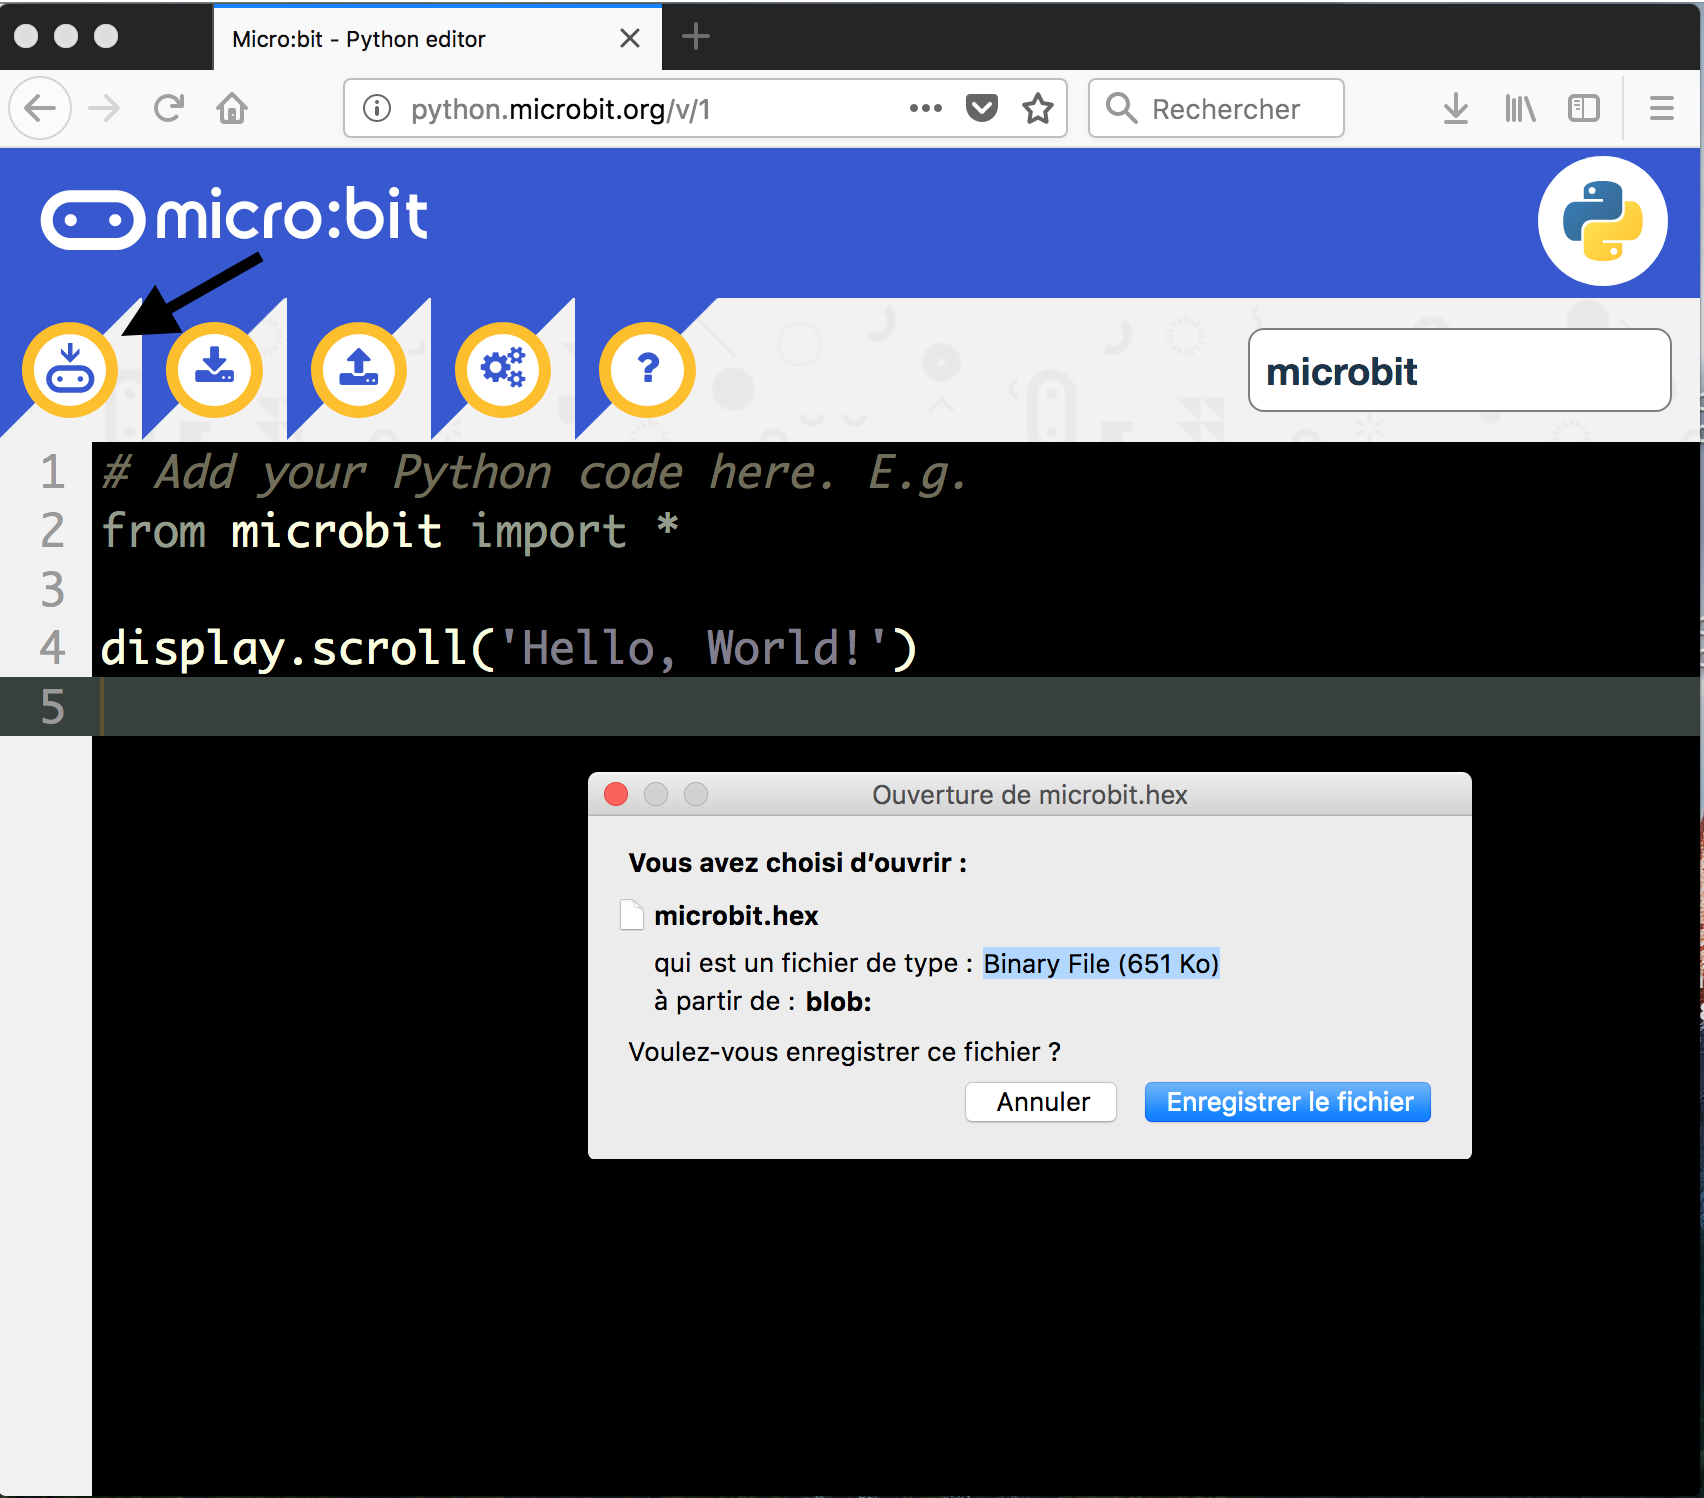
\includegraphics[width=0.45\textwidth]{editeur_compilateur}
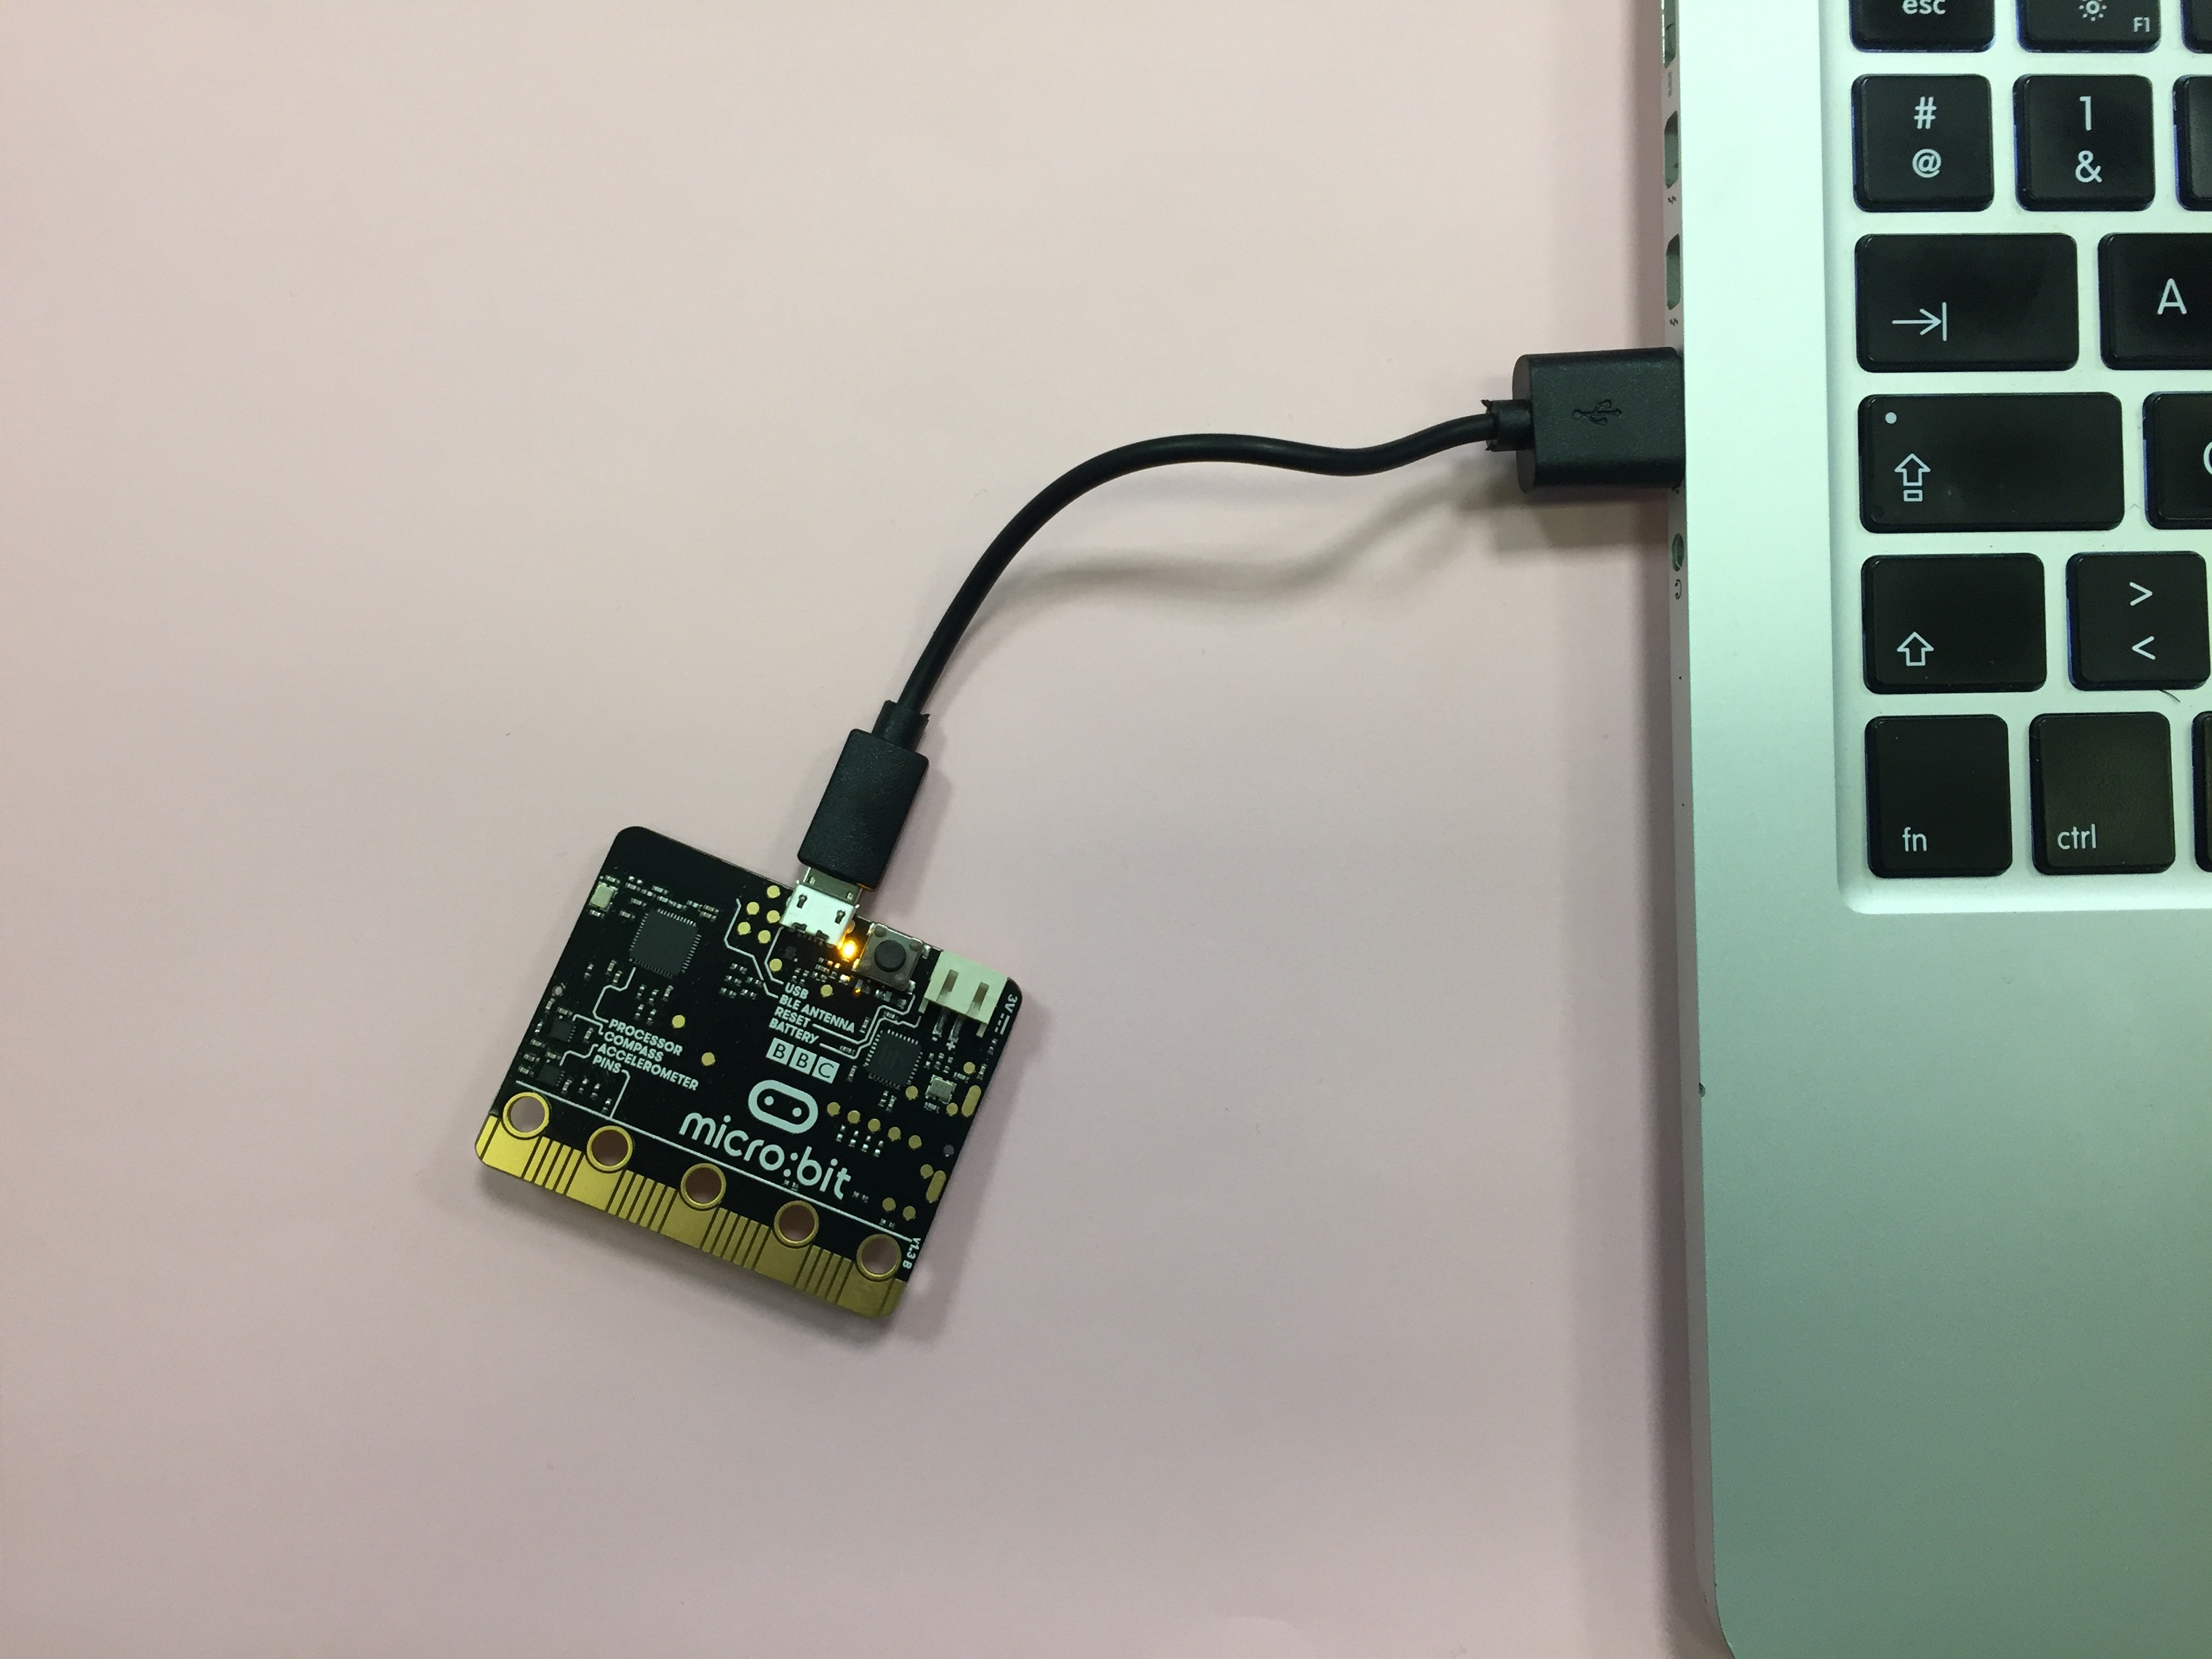
\includegraphics[width=0.45\textwidth]{microbit_telechargement}\\
\end{center}


\partie{Programmer des conditions simples} \\ %{{{1
Si nous voulons que MicroPython réagisse aux événements de presse de bouton, nous devrions le placer dans une boucle infinie et vérifier si le bouton est \texttt{is\_pressed()}.\\

\begin{lstlisting}
from microbit import *

while True:
    if button_a.is_pressed():
        display.show(Image.HAPPY)
\end{lstlisting}

\question Que fait ce programme ?
\reponse
\reponse

\question Peut-on faire autre chose qu'effacer l'image en appuyant sur le boton RESET ?
\reponse
\reponse

\begin{lstlisting}
from microbit import *

while True:
    if button_a.is_pressed():
        display.show(Image.HAPPY)
    else:
	display.clear()
\end{lstlisting}

\question Que fait ce programme ?
\reponse
\reponse

\begin{lstlisting}
from microbit import *

while True:
    if button_a.is_pressed():
        display.show(Image.HAPPY)
    else:
        display.show(Image.SAD)
\end{lstlisting}

\question Que fait ce programme ?
\reponse
\reponse

\begin{lstlisting}
from microbit import *

while True:
    if button_a.is_pressed():
        display.show(Image.HAPPY)
    elif button_b.is_pressed():
        display.show(Image.SAD)
    else:
	display.clear()
\end{lstlisting}

\question Que fait ce programme ?
\reponse
\reponse

\begin{lstlisting}
from microbit import *

while True:
    if button_a.is_pressed():
        display.show(Image.HAPPY)
    elif button_b.is_pressed():
        display.show(Image.SAD)
\end{lstlisting}

\question Que fait ce programme ?
\reponse
\reponse

\begin{lstlisting}
from microbit import *

while True:
    if button_a.is_pressed():
        display.show(Image.HAPPY)
    if button_b.is_pressed():
        display.show(Image.SAD)
\end{lstlisting}

\question Que fait ce programme ?
\reponse
\reponse


%}}}

\bigskip

\partie{Programmer des conditions plus évoluées} \\%{{{1
Reprennez le programme suivant :
\begin{lstlisting}
from microbit import *

while True:
    if button_a.is_pressed():
        display.show(Image.HAPPY)
    if button_b.is_pressed():
        display.show(Image.SAD)
\end{lstlisting}

\question Que fait ce programme quand on appuie sur les deux boutons en même temps ?
\reponse
\reponse

\begin{lstlisting}
from microbit import *

while True:
    if button_a.is_pressed():
        display.show(Image.HAPPY)
    elif button_b.is_pressed():
        display.show(Image.SAD)
\end{lstlisting}

\question Et que fait le programme que nous avons déjà vu quand on appuie sur les deux boutons en même temps ?
\reponse
\reponse

\begin{lstlisting}
from microbit import *

while True:
    if button_a.is_pressed():
        display.show(Image.HAPPY)
        if button_b.is_pressed():
            display.show(Image.SAD)
\end{lstlisting}

\question Que fait ce programme ?
\reponse
\reponse

\question Que fait ce programme quand on appuie sur les deux boutons en même temps ?
\reponse
\reponse

\begin{lstlisting}
from microbit import *

while True:
    if button_a.is_pressed():
        display.show(Image.HAPPY)
    if button_b.is_pressed():
        display.show(Image.SAD)
    else:
	display.clear()
\end{lstlisting}

\question Que fait ce programme ?
\reponse
\reponse

\question Que fait ce programme quand on appuie sur les deux boutons en même temps ?
\reponse
\reponse

Maintenant, faisons un cyber-animal très simple. Il est toujours triste à moins d'appuyer sur le bouton A. Si vous appuyez sur le bouton B il disparaît.
\begin{lstlisting}
from microbit import *

while True:
    if button_a.is_pressed():
        display.show(Image.HAPPY)
    elif button_b.is_pressed():
        break
    else:
        display.show(Image.SAD)
display.clear()
\end{lstlisting}

\question Que fait la fonction break ?
\reponse
\reponse

\question Quelle ligne de code est donc exécutée ensuite ?
\reponse

\question Décrire ce programme ligne à ligne ?
\reponse
\reponse
\reponse
\reponse

\question Après avoir appuyé le bouton b, peut-on à nouveau faire apparaître le visage HAPPY ?
\reponse

%}}}

\bigskip

\partie{Programmer une entrée plutôt originale} \\ %{{{1
Pour faire marcher le programme suivant, il suffit en principe de toucher la pin 0. En pratique, ce la aide de prendre avec la main droite la pin GND ou masse, et pincer la pin 0 avec la main gauche. Ca marche presque à tout les coups : insister un peu vaut le coup. \\
\begin{lstlisting}
from microbit import *

while True:
    if pin0.is_touched():
        display.show(Image.HAPPY)
    else:
        display.show(Image.SAD)
\end{lstlisting}

\question Décrire ce programme ligne à ligne ?
\reponse
\reponse
\reponse
%}}}

\bigskip

\partie{Mouvement}\\ %{{{1
Le micro:bit est livré avec un accéléromètre. Il mesure le mouvement selon trois axes:\\
X - inclinaison de gauche à droite.\\
Y - inclinaison vers l'avant et vers l'arrière.\\
Z - se déplaçant de haut en bas.
\begin{lstlisting}
from microbit import *

while True:
    reading = accelerometer.get_x()
    if reading > 20:
        display.show("R")
    elif reading < -20:
        display.show("L")
    else:
        display.show("-")
\end{lstlisting}

\question Décrire ce programme ligne à ligne ?
\reponse
\reponse

\question Que changer dans ce programme pour que l'on voit le caractère "-" plus souvent ?
\reponse

%}}}


\end{document}
% vim:fdl=0
